\section{Introduction}

With the incredible advancement of high resolution neural recording, manipulation technology and computing power, the amount of data for both experimental and simulated neural population activity is increasing tremendously and can be quite overwhelming, for both analysis, interpretation and theory construction. Computational and analytical tools to interpret and build models from such volumes of data for hypothesis testing and exploratory purposes are catching up. Tools like topological data analysis (TDA) and network analysis inevitably are necessary for extracting and exploring potential structures and patterns within these data. Over the last two decades, there have been multiple applications of algebraic topology tools in neuroscience, extending analysis from traditional graph theory and network science methods. Aside from the more theoretical endeavors, these applications peruse TDA in neural population data across different subfields of computational neuroscience, most of which involve clique topology analysis. Examples span across different data domains and areas, from electrophysiological recordings in a specific area \cite{Giusti2015-uo} (rodent hippocampal place cells), to brain-wide structural human connectome \cite{Sizemore2018-ql}, as well as within detailed biophysical neural simulations and models \cite{Reimann2017-ji}. Although there have been quite many population studies across other areas like neocortex, subcortical areas and hippocampus, not many network studies are done in the cerebellar Purkinje population recordings, even though these cells are among the popular neurons usually shown in textbooks with their beautiful complicated morphology, responsible for many developmental and learning functions such as motor learning. To my knowledge, there are no studies to date applying TDA in the cerrebellum population data.

\begin{figure}[H]
    \centering
    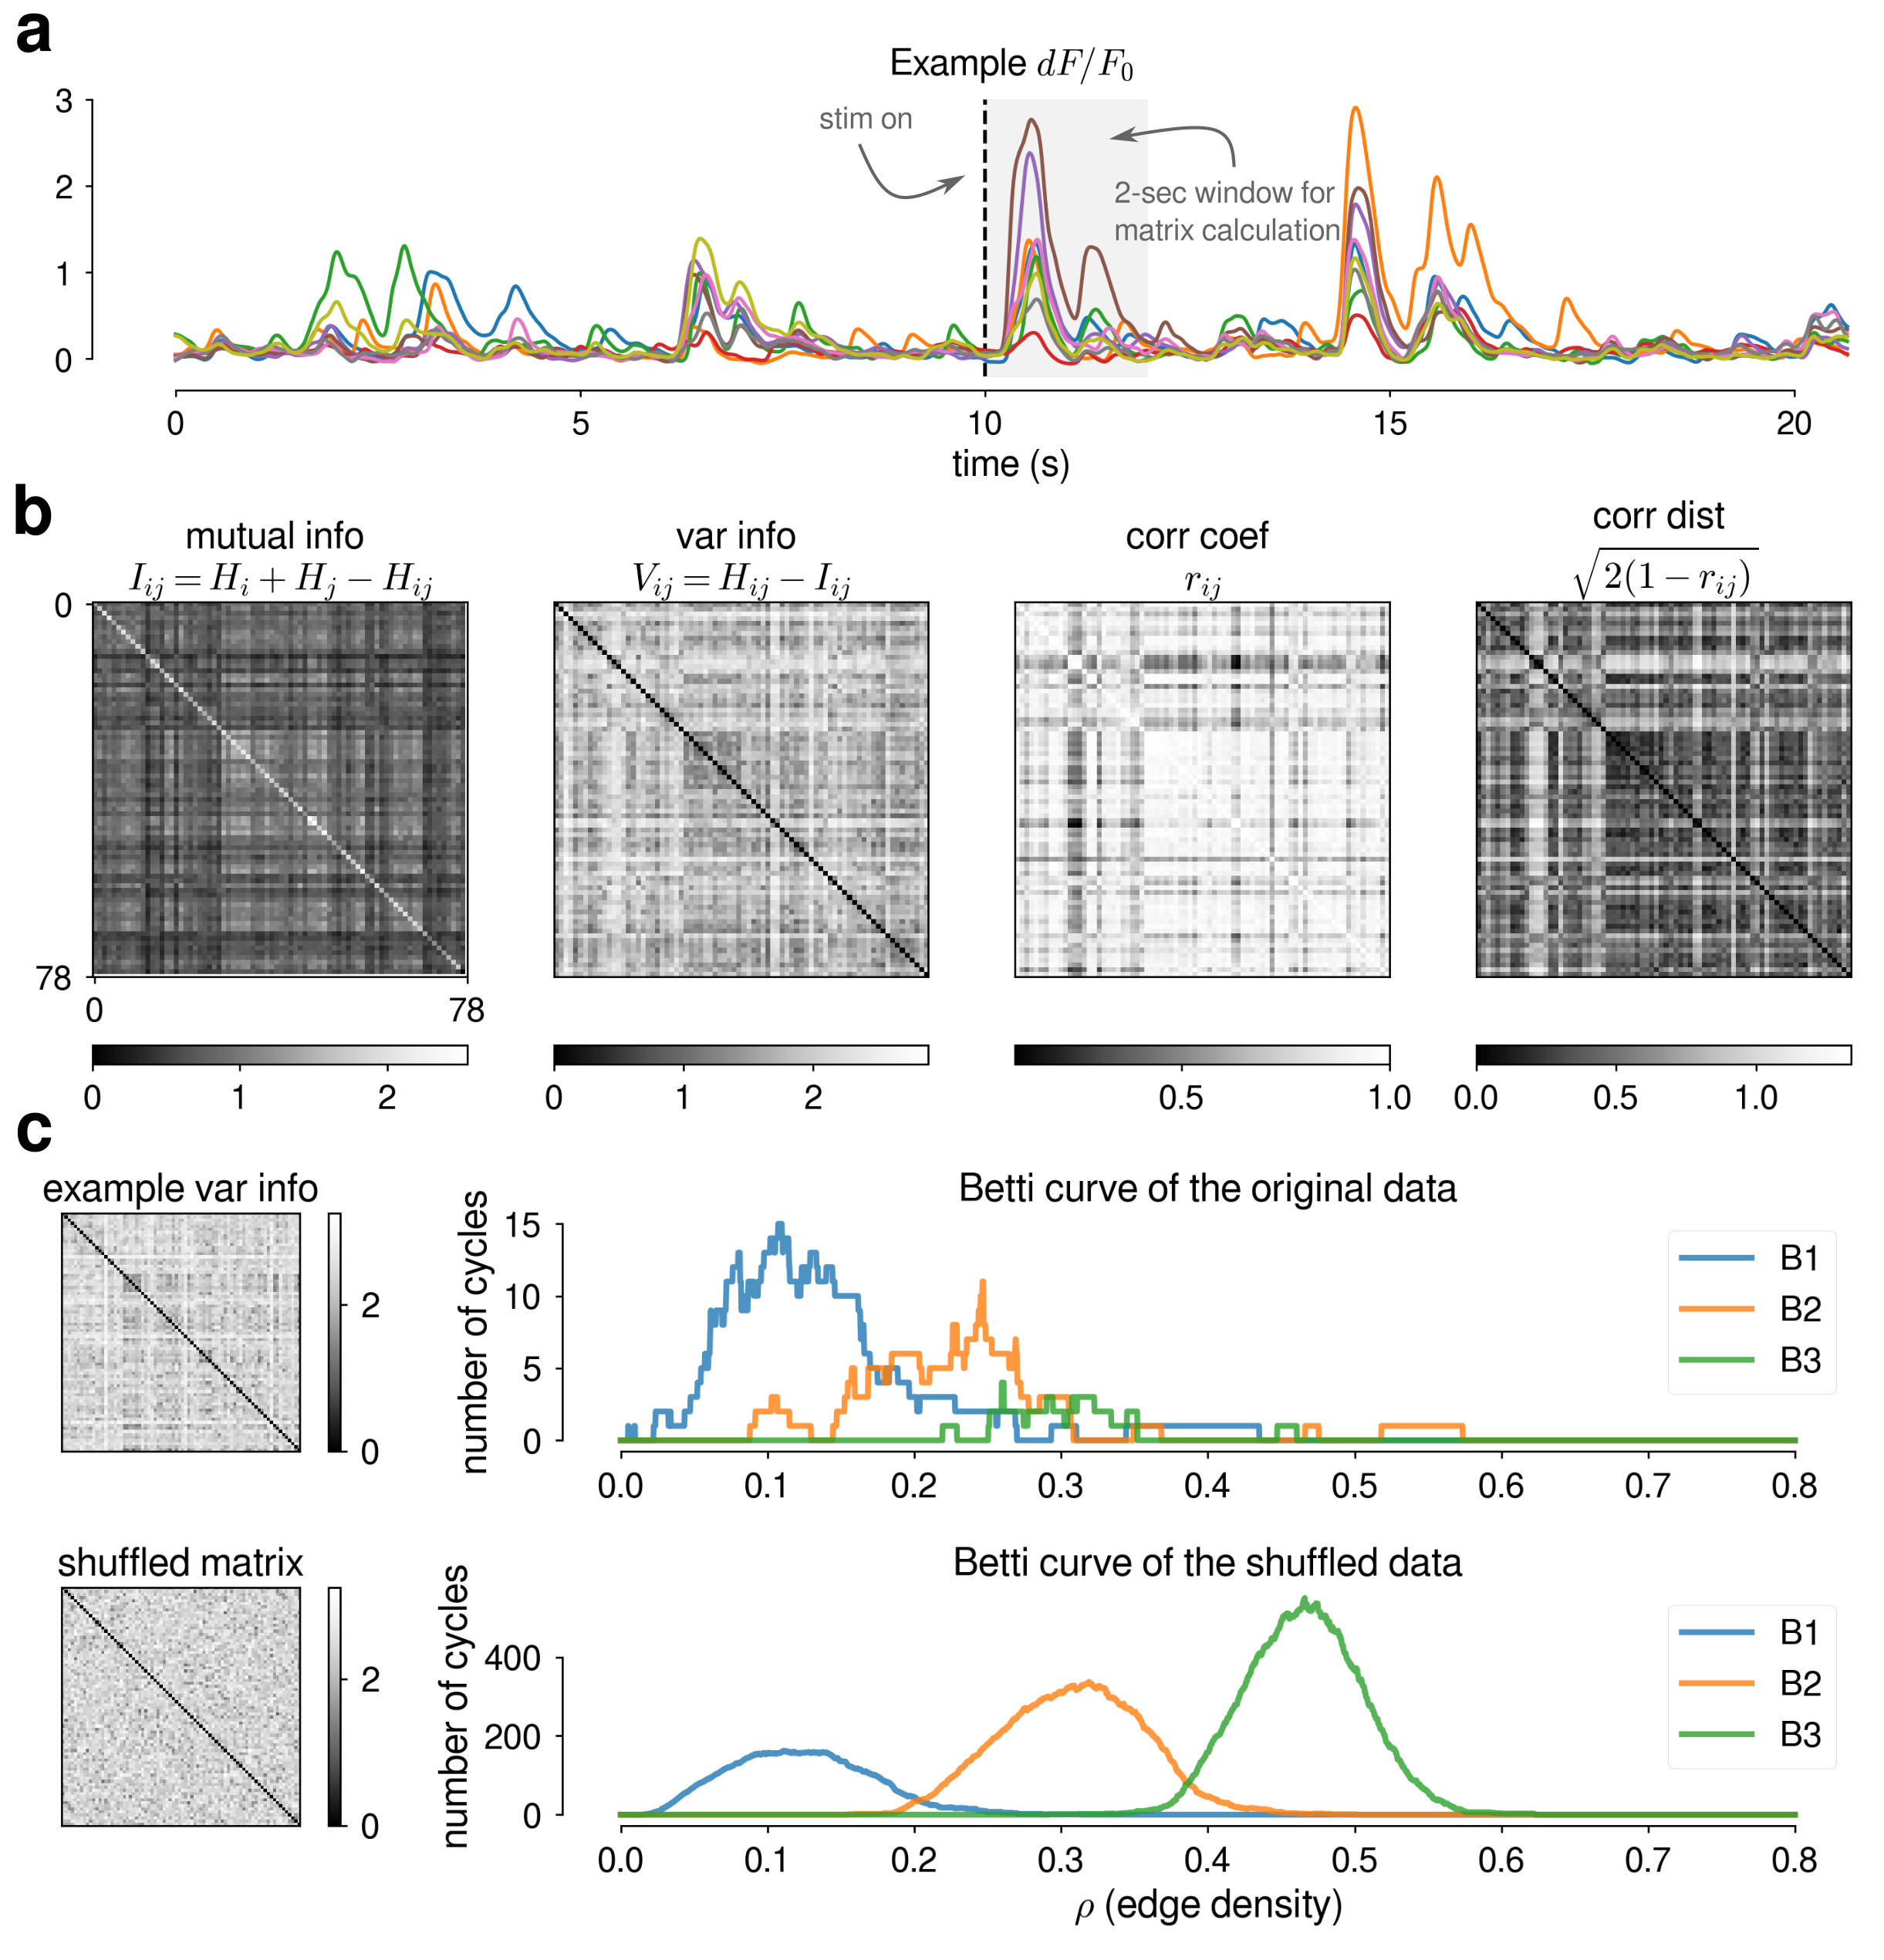
\includegraphics[width=0.5\textwidth,center]{../figures/report/Fig1.png}
    \caption{\label{fig:1}
    \textit{Title}.
    Descriptions
    }
\end{figure}


Hence, I want to apply TDA on Purkinje cell population and drawing comparison with different models of random graphs, similar to \cite{Giusti2015-uo}. More specifically, I based my project around the ideas and methods from \cite{Giusti2015-uo}, which shows the geometric organization in hippocampal correlation structure across different states of the animal, including during wheel-running behavior and sleep. This was accomplished by comparing the Betti number curves by analyzing the homology of order complex between the data and those from generated random geometric networks, as well as comparing with a null based on shuffled data. In addition to comparison between the population and different null models, including geometric and block models, because the data are associated with different brief evoked sensory stimulus conditions, I explored how these different sensory modalities affect the topology features of the network. Moreover, I examined whether it is possible to classify the stimulus categories either from the topology features alone, or with combination of activity data.